% figure-3-posets-that-are-not-plotkin-orders.tex
%
% Source:   Carl A. Gunter and Dana S. Scott, "Semantic Domains" (1990).
%           ScottDomains/papers/Gunter Scott 1990.pdf
% Physical page: 32          Printed page: 31
% Section:  6. Bifinite domains, immediately after Theorem 14 and before
%           subsection 6.2 "Closure properties".
% Caption (verbatim):  "Figure 3: Posets that are not Plotkin orders."
%
% Introducing sentences (printed page 30 / physical page 31, and printed
% page 31 / physical page 32):
%   "This rules out configurations like the one pictured in Figure 3a where
%    the pair of points indicated by closed circles do not have such a
%    complete set of minimal upper bounds."
%   "This rules out configurations like the one pictured in Figure 3b where
%    the pair of points indicated by closed circles has a complete set of
%    minimal upper bounds but not a finite one."
%   "To see what can go wrong, note that U^\infty(u) is infinite when u is
%    the pair of points indicated by closed circles in Figure 3c."
%
% Reading of the three parts:
%   a.  The two closed points have upper bounds forming an infinite DESCENDING
%       chain of open circles, so no upper bound is minimal: no complete set
%       of minimal upper bounds exists.
%   b.  The two closed points have infinitely many minimal upper bounds (the
%       row of open circles, continuing left and right), so the complete set
%       of minimal upper bounds is not finite.
%   c.  Every finite subset has a finite complete set of minimal upper bounds,
%       but the mub-closure U^\infty of the closed pair is infinite: the
%       two-column ladder repeats upward without end.
%
% The closed (filled) circles are the distinguished pair u in every part;
% that distinction is the whole content of the paper's discussion, so it is
% preserved here and must never be flattened to a uniform vertex mark.
%
% Geometry was measured from 600 dpi crops of physical page 32 and mapped to
% centimetres by (page pixel - 748)/200 horizontally and (2347 - page
% pixel)/200 vertically, so the three parts keep their relative placement,
% scale and truncated-edge slopes.
%
% Deviation from the r0039 style contract: the contract's line
% "\usetikzpicture{}" is a typo - no such macro exists - and is dropped here.
% No extra TikZ library is needed.

\documentclass[border=6pt]{standalone}
\usepackage{tikz}
\begin{document}
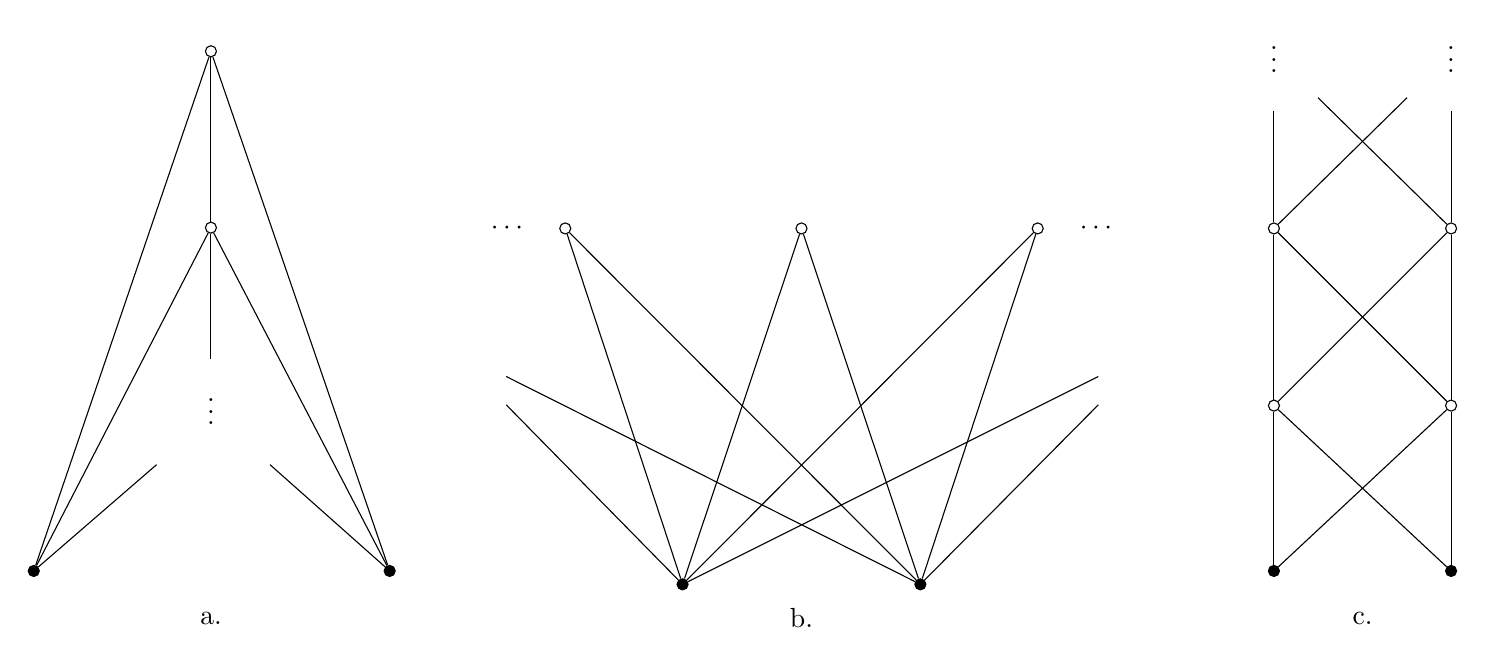
\begin{tikzpicture}[
  x=1cm, y=1cm,
  every node/.style={inner sep=1pt},
  open/.style={circle, draw, fill=white, minimum size=4pt, inner sep=0pt},
  solid/.style={circle, draw, fill=black, minimum size=4pt, inner sep=0pt},
  edge/.style={draw, line width=0.4pt}]

  %% ---------------- part a ----------------
  % vertices
  \node[solid] (aL) at (0.00, 0.00) {};
  \node[solid] (aR) at (4.52, 0.00) {};
  \node[open]  (u2) at (2.25, 4.36) {};
  \node[open]  (u1) at (2.25, 6.60) {};
  % edges
  \draw[edge] (u1) -- (u2);
  \draw[edge] (u1) -- (aL);
  \draw[edge] (u1) -- (aR);
  \draw[edge] (u2) -- (aL);
  \draw[edge] (u2) -- (aR);
  % the chain continues downward: stub below u2, then the vertical ellipsis
  \draw[edge] (u2) -- (2.25, 2.69);
  \node at (2.25, 2.13) {$\vdots$};
  % truncated edges from the next chain element (below the ellipsis)
  \draw[edge] (aL) -- (1.56, 1.35);
  \draw[edge] (aR) -- (3.00, 1.35);
  % part label
  \node at (2.25, -0.60) {a.};

  %% ---------------- part b ----------------
  % vertices
  \node[solid] (bL) at (8.24, -0.17) {};
  \node[solid] (bR) at (11.26, -0.17) {};
  \node[open]  (m1) at (6.75, 4.35) {};
  \node[open]  (m2) at (9.75, 4.35) {};
  \node[open]  (m3) at (12.75, 4.35) {};
  % edges
  \draw[edge] (m1) -- (bL);
  \draw[edge] (m1) -- (bR);
  \draw[edge] (m2) -- (bL);
  \draw[edge] (m2) -- (bR);
  \draw[edge] (m3) -- (bL);
  \draw[edge] (m3) -- (bR);
  % the row of minimal upper bounds continues left and right
  \node at (6.01, 4.35) {$\cdots$};
  \node at (13.49, 4.35) {$\cdots$};
  % truncated edges to the off-picture minimal upper bounds
  \draw[edge] (bL) -- (6.00, 2.11);
  \draw[edge] (bR) -- (6.00, 2.47);
  \draw[edge] (bL) -- (13.52, 2.47);
  \draw[edge] (bR) -- (13.52, 2.11);
  % part label
  \node at (9.75, -0.60) {b.};

  %% ---------------- part c ----------------
  % vertices
  \node[solid] (cBL) at (15.75, 0.00) {};
  \node[solid] (cBR) at (18.00, 0.00) {};
  \node[open]  (cML) at (15.75, 2.10) {};
  \node[open]  (cMR) at (18.00, 2.10) {};
  \node[open]  (cTL) at (15.75, 4.35) {};
  \node[open]  (cTR) at (18.00, 4.35) {};
  % edges: each level is joined to the next by a complete bipartite K_{2,2}
  \draw[edge] (cBL) -- (cML);
  \draw[edge] (cBL) -- (cMR);
  \draw[edge] (cBR) -- (cMR);
  \draw[edge] (cBR) -- (cML);
  \draw[edge] (cML) -- (cTL);
  \draw[edge] (cML) -- (cTR);
  \draw[edge] (cMR) -- (cTR);
  \draw[edge] (cMR) -- (cTL);
  % truncated edges into the next level up, then the vertical ellipses
  \draw[edge] (cTL) -- (15.75, 5.84);
  \draw[edge] (cTR) -- (18.00, 5.84);
  \draw[edge] (cTL) -- (17.44, 6.01);
  \draw[edge] (cTR) -- (16.31, 6.01);
  \node at (15.75, 6.60) {$\vdots$};
  \node at (18.00, 6.60) {$\vdots$};
  % part label
  \node at (16.875, -0.60) {c.};

\end{tikzpicture}
\end{document}
